%\documentclass[t]{beamer}  % [t], [c], или [b] --- вертикальное выравнивание на слайдах (верх, центр, низ)
\documentclass{beamer} % Соотношение сторон

%графики
\usepackage{pgfplots}
\pgfplotsset{compat=1.9}

\usetheme{Madrid}
\usefonttheme{serif}



%%% Работа с русским языком
\usepackage[T2A]{fontenc}			% кодировка
\usepackage[utf8]{inputenc}			% кодировка исходного текста
\usepackage[english,russian]{babel}	% локализация и переносы
%%% Дополнительная работа с математикой
\usepackage{amsmath,amsfonts,amssymb,amsthm,mathtools} % AMS
\usepackage{bm}

%%% Работа с картинками
\usepackage{graphicx}  % Для вставки рисунков
\setlength\fboxsep{3pt} % Отступ рамки \fbox{} от рисунка
\setlength\fboxrule{1pt} % Толщина линий рамки \fbox{}

\usepackage{braket} %Бракеты
\usepackage[version=4]{mhchem} 

\newtheorem{thrm}{Теорема}

\title[]{Капельница Кельвина}

\subtitle{}
\author{Калиничев И. и Адамян Г.}
\institute[МФТИ]{МФТИ \newline ФОПФ}
\renewcommand{\arraystretch}{1.3}

\setbeamersize{text margin left=20pt,text margin right=20pt}

\usepackage{pgfpages}
%\pgfpagesuselayout{2 on 1}[a4paper,border shrink=5mm]

\begin{document}

\frame[plain]{\titlepage}	% Титульный слайд

\section{проблема}
%%%%%%%%%%%%%%%%%%%%%%%%%%%%%%%%%%%%%%%%%%%%%%%%%%%%%%%%%%%%%%%%%%
%% 2 %%
\begin{frame}[c]
	\frametitle{Устройство установки}
	\begin{figure}[h]

\centering

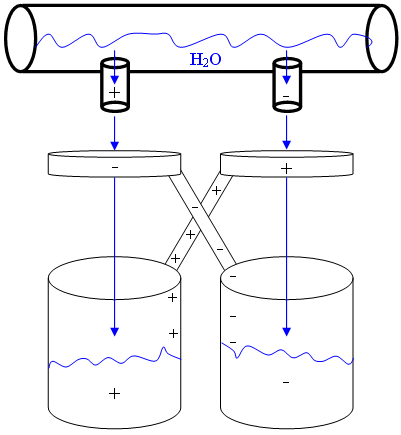
\includegraphics[width=0.5\linewidth]{Kelvin_water_dropper.png}

\caption{Схема капельницы}

\label{fig:mpr}

\end{figure}
\end{frame}
%%%%%%%%%%%%%%%%%%%%%%%%%%%%%%%%%%%%%%%%%%%%%%%%%%%%%%%%%%%%%%%%%%

%% 3 %%
\begin{frame}[c]
	\frametitle{Идеальное расстояние до цилиндров}
	\centering
	\begin{figure}[h]

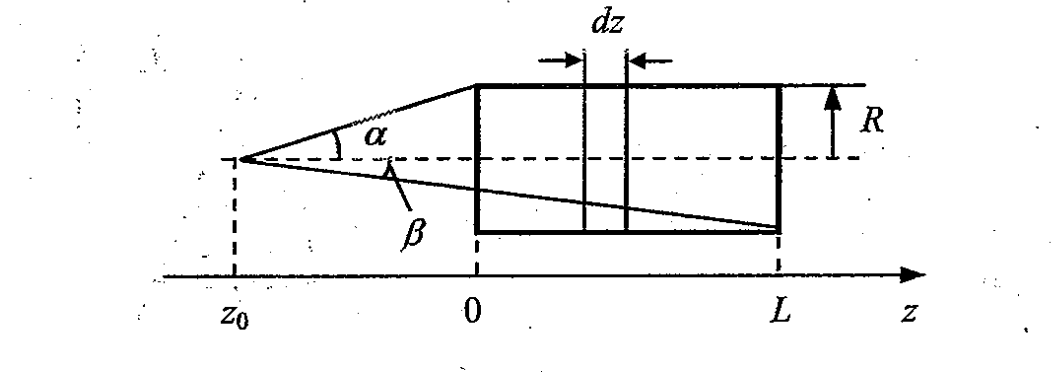
\includegraphics[width=0.8\linewidth]{vpv_cilindr.png}
\label{fig:mpr}

\end{figure}
$$E = \int{dE} = \int{\frac{dq}{(z+z_0)^2}}$$
$$dq = \sigma \cdot  2\pi R \ dz$$
$$\sin \varphi \  dz = \frac{R}{\sin \varphi} \  d\varphi \Rightarrow dz = \frac{R}{\sin^2\varphi} \ d\varphi$$
$$z-z_0 = \frac{R}{sin\varphi}$$
\end{frame}
%%%%%%%%%%%%%%%%%%%%%%%%%%%%%%%%%%%%%%%%%%%%%%%%%%%%%%%%%%%%%%%%%%

%% 4 %%
\begin{frame}[c]
	\frametitle{Идеальное расстояние до цилиндров}
	\centering

\centering
$$E = \int\limits_\alpha^\beta{\frac{2 \pi R \sigma dz}{R^2} \ \sin^2 \varphi \ \cos \varphi} = \int\limits_\alpha^\beta{2 \pi \sigma \cos \varphi \ d\varphi}$$
$$E = 2 \pi \sigma (\sin \alpha - \sin \beta)$$
$$\sin \alpha = \frac{R}{\sqrt{R^2+z_0^2}}$$
$$\sin \beta = \frac{R}{\sqrt{R^2+(L+z_0)^2}}$$
$$E = 2 \pi \sigma \bigg( \frac{R}{\sqrt{R^2+z_0^2}} - \frac{R}{\sqrt{R^2+(L+z_0)^2}} \bigg)$$

\end{frame}
%%%%%%%%%%%%%%%%%%%%%%%%%%%%%%%%%%%%%%%%%%%%%%%%%%%%%%%%%%%%%%%%%%
%% 5 %%
\begin{frame}[c]
	\frametitle{Идеальное расстояние до цилиндров}
	\centering
\begin{figure}[h]

\centering

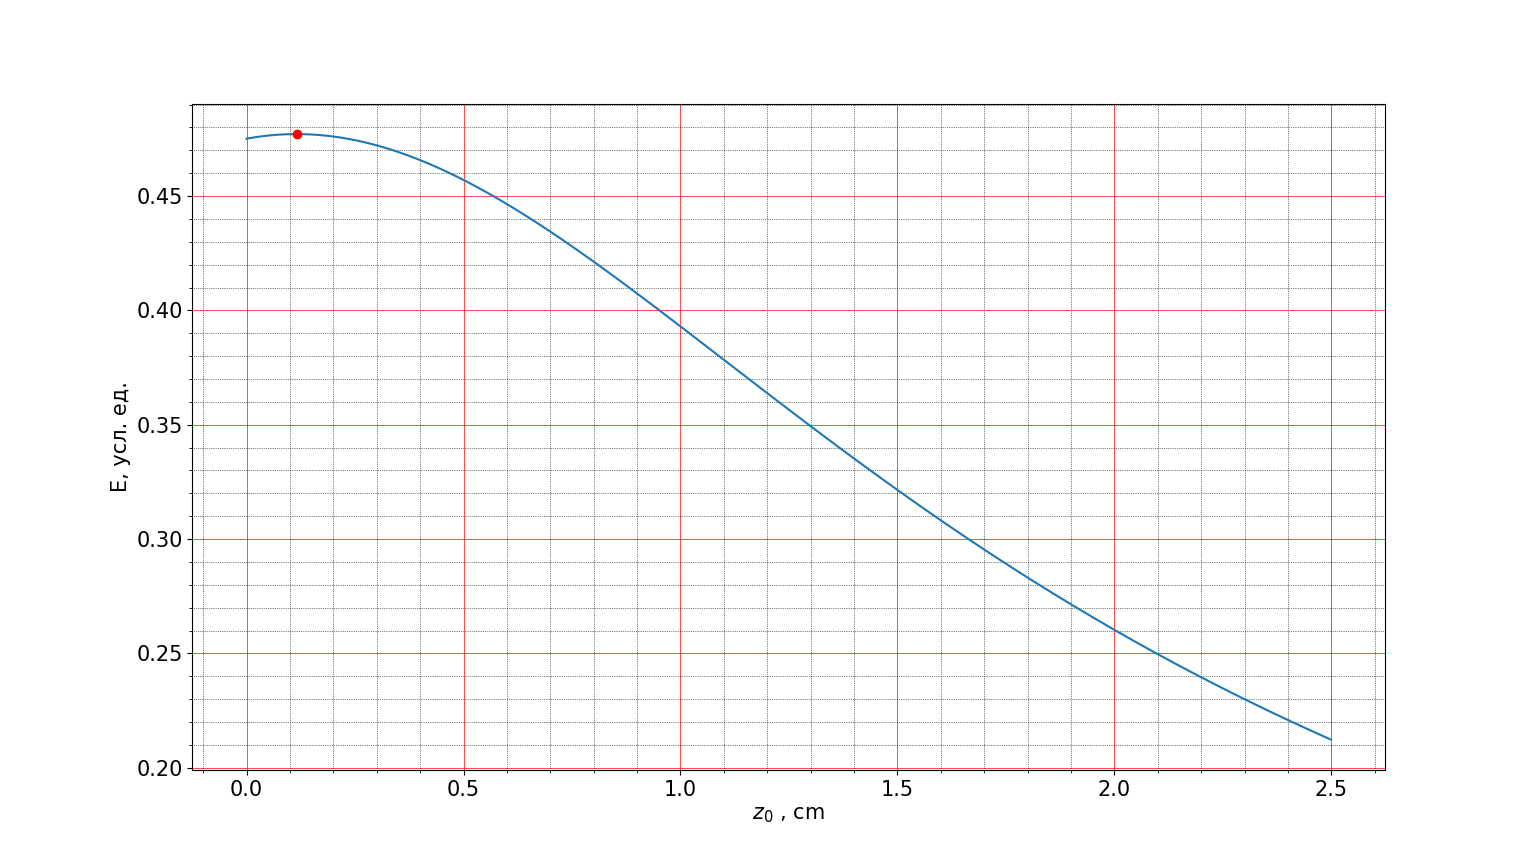
\includegraphics[width=0.8\linewidth]{vpv_E.png}

\caption{Зависимость поля от расстояния до цилиндра}
\label{fig:mpr}

\end{figure}
\end{frame}
%%%%%%%%%%%%%%%%%%%%%%%%%%%%%%%%%%%%%%%%%%%%%%%%%%%%%%%%%%%%%%%%%%

%% 6 %%
\begin{frame}[c]
	\frametitle{Немного теории про электролиты}
	\centering
\begin{figure}[h]

\centering

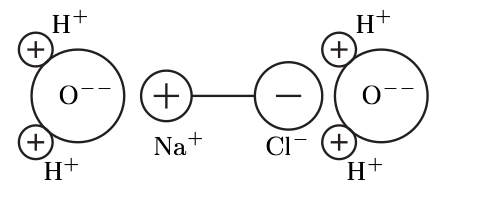
\includegraphics[width=0.6\linewidth]{vpv_ions.png}

\caption{Появление ионов в воде}
\label{fig:mpr}

\end{figure}
\end{frame}
%%%%%%%%%%%%%%%%%%%%%%%%%%%%%%%%%%%%%%%%%%%%%%%%%%%%%%%%%%%%%%%%%%

%% 7 %%
\begin{frame}[c]
	\frametitle{Результат эксперимента}
	\centering
\begin{figure}[h]

\centering

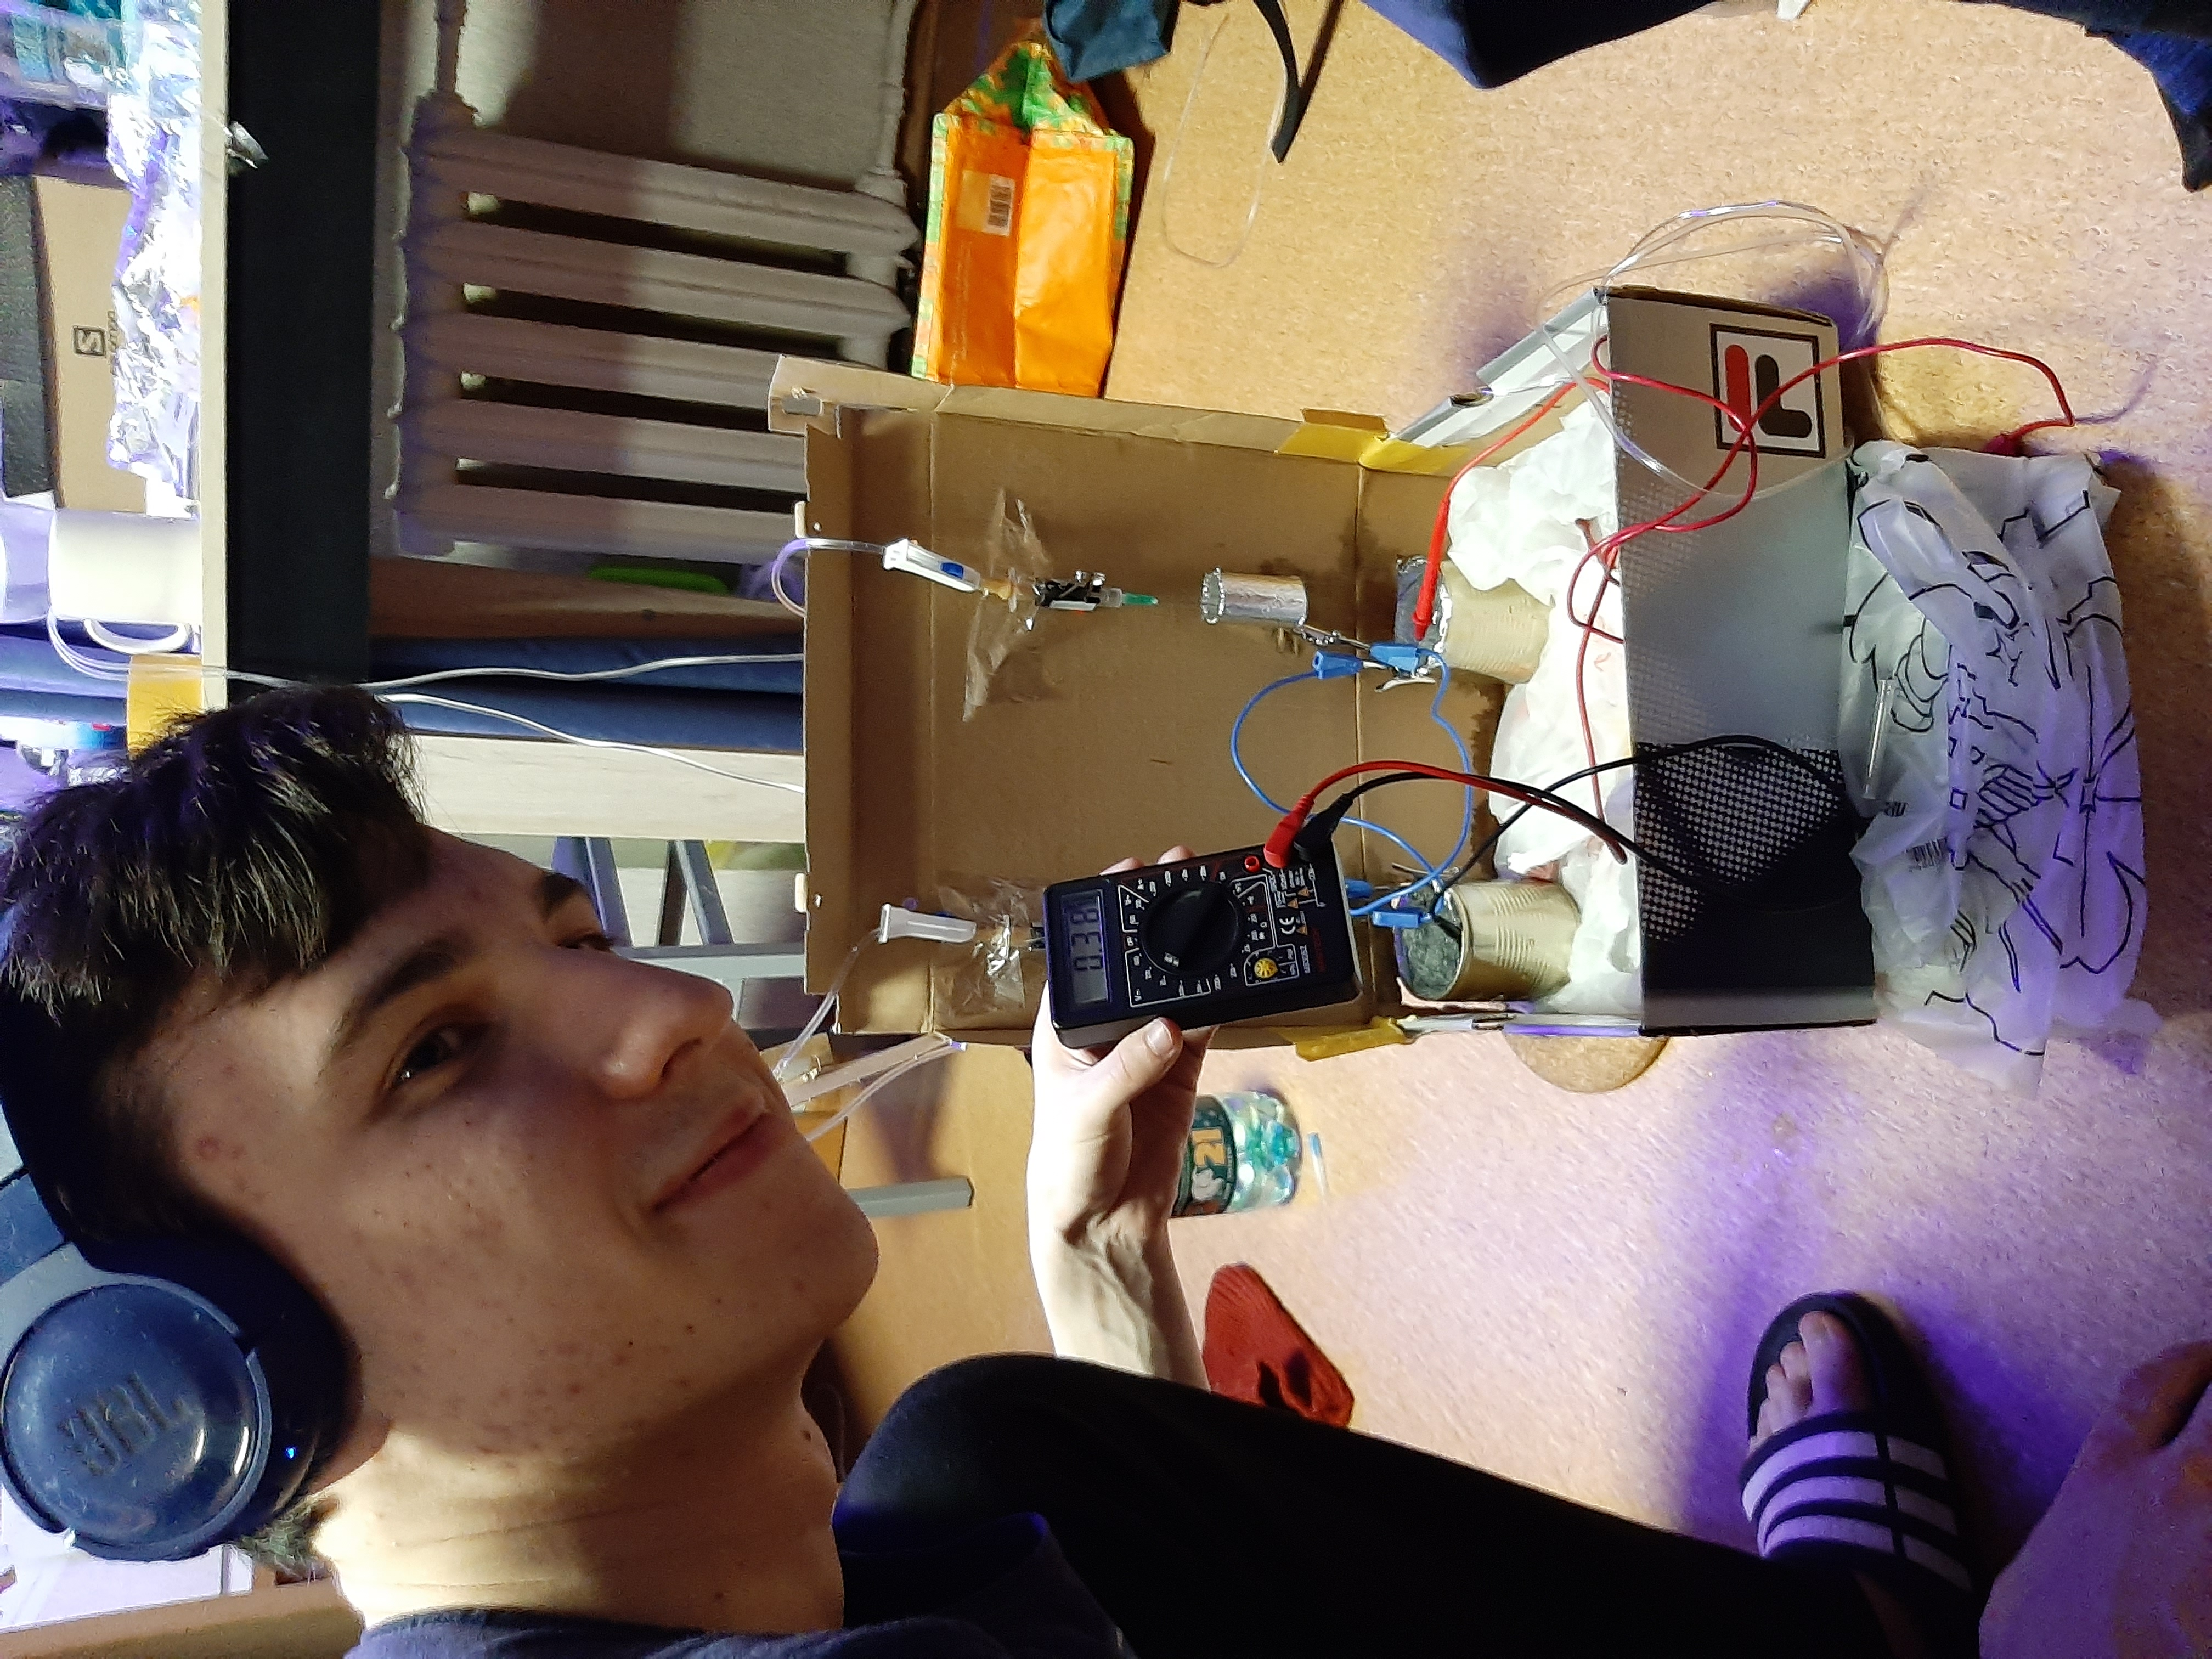
\includegraphics[width=0.5\linewidth]{vpv_Igor.png}

\label{fig:mpr}

\end{figure}
\end{frame}
%%%%%%%%%%%%%%%%%%%%%%%%%%%%%%%%%%%%%%%%%%%%%%%%%%%%%%%%%%%%%%%%%%


\end{document}
